\documentclass[../main.tex]{subfile}

\begin{document}

\section{Séparation nette}

La communication intensive des aspects du film au spectateur est une des grande
écoles du cinéma. C'est d'ailleurs comme cela que le cinéma s'est lancé, se
basant avant tout sur des documentaires avant de passer au stade
divertissement. C'est pourquoi à une époque même la fiction au cinéma était
narrée précisément.

Dans le cas du rêve, et au vu de la difficulté de différencier le monde du rêve
et celui de la réalité au sein d'un film, communiquer au spectateur semble être
une méthode brutale mais efficace.

Le risque dans cette situation est de \textbf{déconnecter} le spectateur de
l'histoire qu'il observe, diminuant ainsi l'effet divertissant du film.

\subsection{Introduction d'éléments contradictoires}

Une méthode très simple et très explicite de séparation nette entre rêve et
réalité au sein d'un film est l'introduction d'éléments contradictoires au
train de l'histoire. On peut notamment citer "Las Vegas Parano" (figure
\ref{fig:images_lasvegas}) qui fait comprendre au spectateur que le personnage
principal est en réalité en plein délire lorsqu'on peut voir que le bar dans
lequel il rentre est rempli de monstres reptiliens, alors qu'ils sont tous des
gens parfaitement normaux depuis un autre point de vue.

\begin{figure}
    \centering
    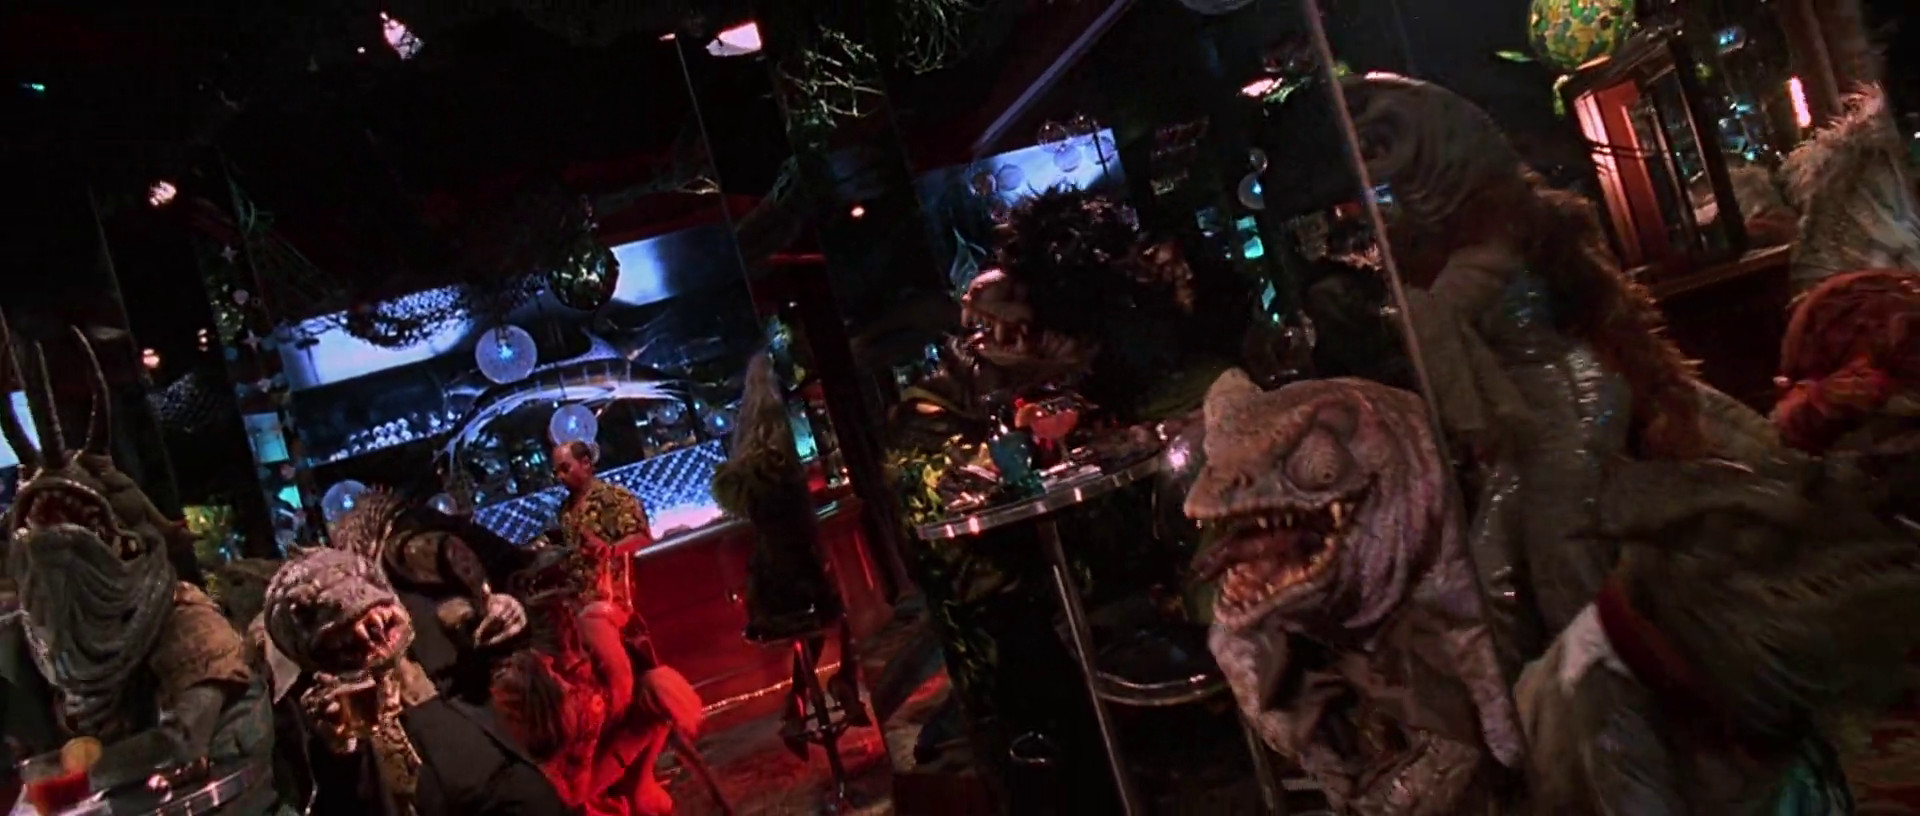
\includegraphics[width=\linewidth]{images/lasvegas}
    \caption{Hallucination du personnage principal, \textit{Las Vegas Parano (1999)}, un film de
             \textit{Terry Gilliam}}
    \label{fig:images_lasvegas}
\end{figure}

\subsection{Surréalisme}

Le surréalisme a toujours été un mouvement intimement lié à l'étude du mondu
onirique. Sa philosophie est d'ailleurs très proche de ce que l'on peut
comprendre d'un rêve : \textit{``Le surréalisme est un automatisme psychique pur,
par lequel on se propose d'exprimer, soit verbalement, soit par écrit, soit de
toute autre manière, le fonctionnement réel de la pensée. Dictée de la pensée,
en l'absence de tout contrôle exercé par la raison, en dehors de toute
préoccupation esthétique ou morale.''} -- André Breton

Certaines techniques du surréalisme sont très appropriées pour montrer au
spectateur la situation souhaitée, tout en incluant des éléments symboliques
attirant l'attention de ce dernier pour ne pas perdre son intérêt.

Dans le cas des films d'animation, le surréalisme est adapté pour l'expression
artistique et est souvent utilisé comme prétexte pour promouvoir l'effort
artistique mis dans la production du dit film. Un exemple évident est le film
"Paprika" (figure \ref{fig:images_paprika}) dont la séparation entre rêve et
réalité peut-être remarqué par une abondance de dessins surréalistes.

\begin{figure}
    \centering
    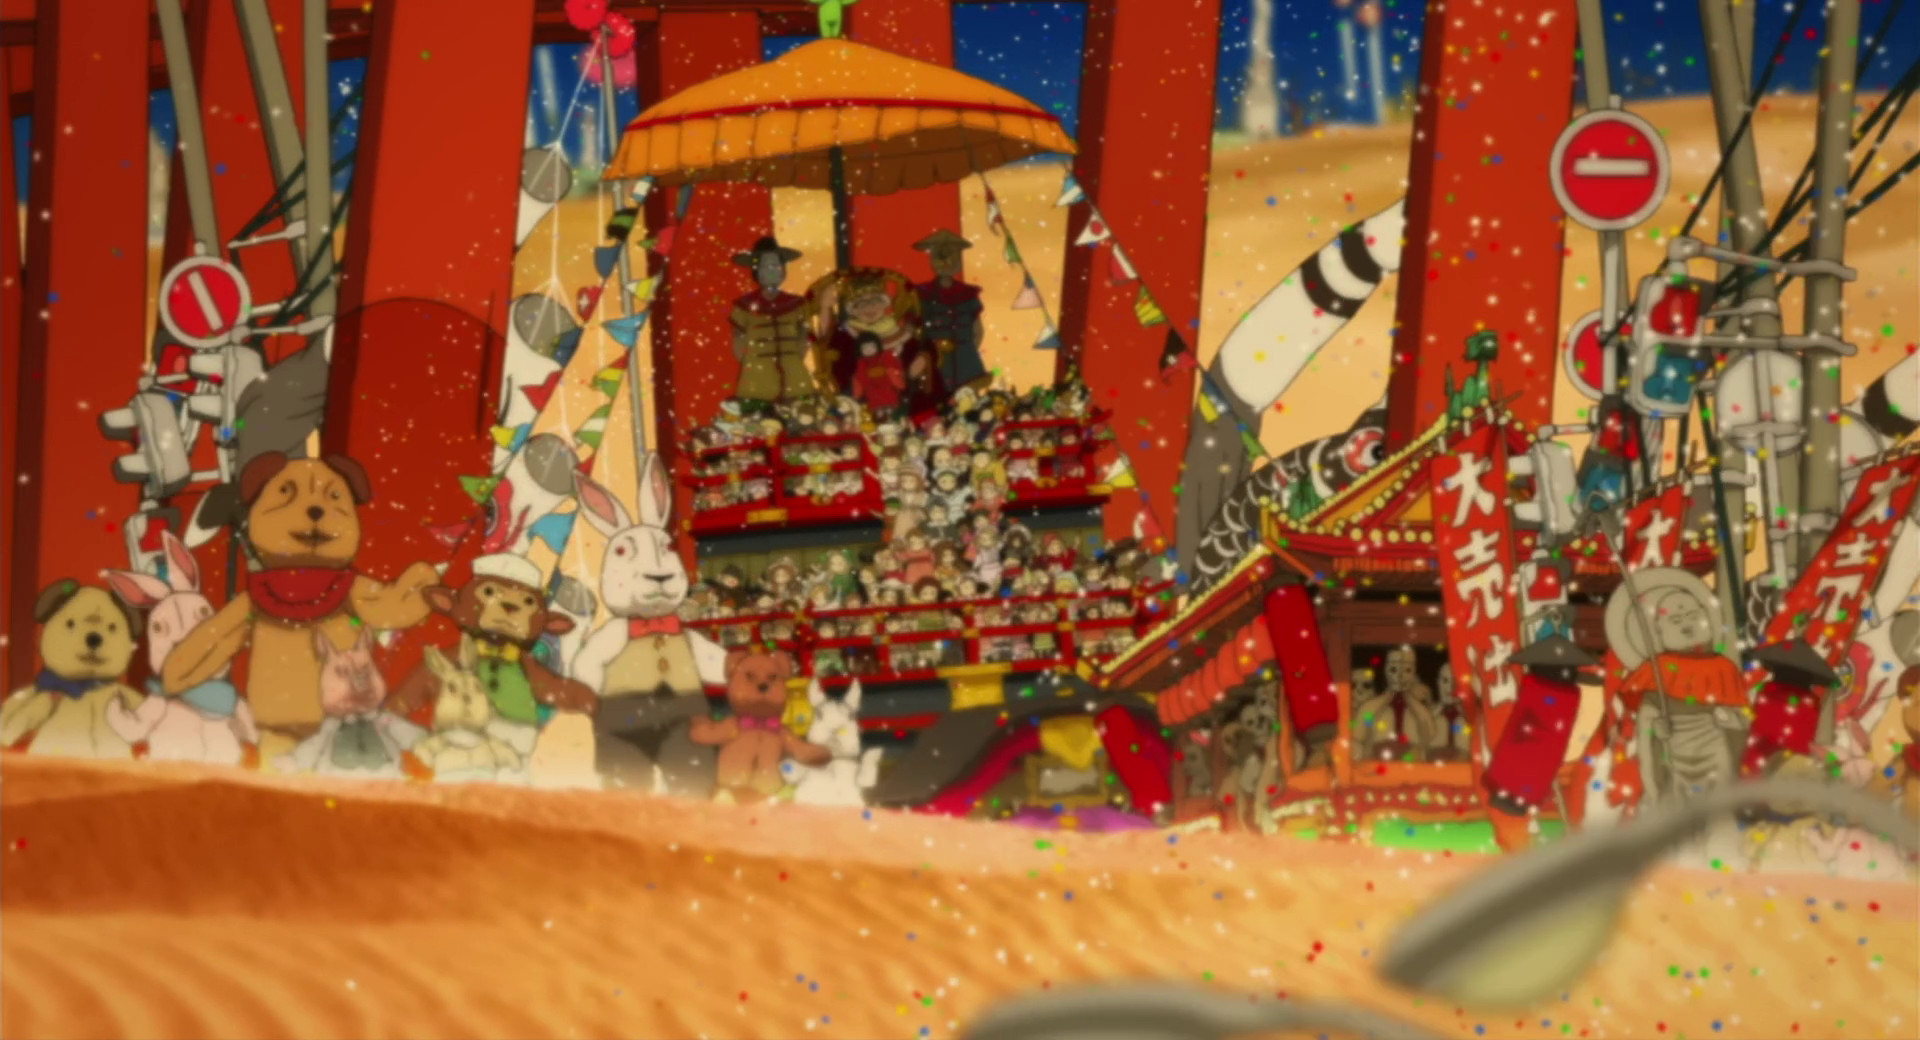
\includegraphics[width=\linewidth]{images/paprika}
    \caption{Surréalisme animé, \textit{Paprika (2006)}, un film de
             \textit{Satoshi Kon}}
    \label{fig:images_paprika}
\end{figure}

\subsection{Erreurs volontaires}

Cela peut paraître paradoxal, mais une des méthodes les plus efficaces pour
montrer la différence entre un rêve et le reste de l'histoire est d'inclure
volontairement des "erreurs", le plus souvent sous la forme de faux-raccords.

La base de la technique est d'éviter de faire des erreurs de ce genre pendant
le reste du film, mais de \emph{casser} le rythme en montrant un élément de
réalisation illogique, tel que la disparition d'un personnage, un changement du
décor en pleine scène, etc...

On peut observer cette méthode dans le film "Scott Pilgrim vs the world"
(figures \ref{fig:images_scott1} et \ref{fig:images_scott2} par exemple).

\begin{figure}
    \centering
    \begin{subfigure}[b]{0.49\textwidth}
        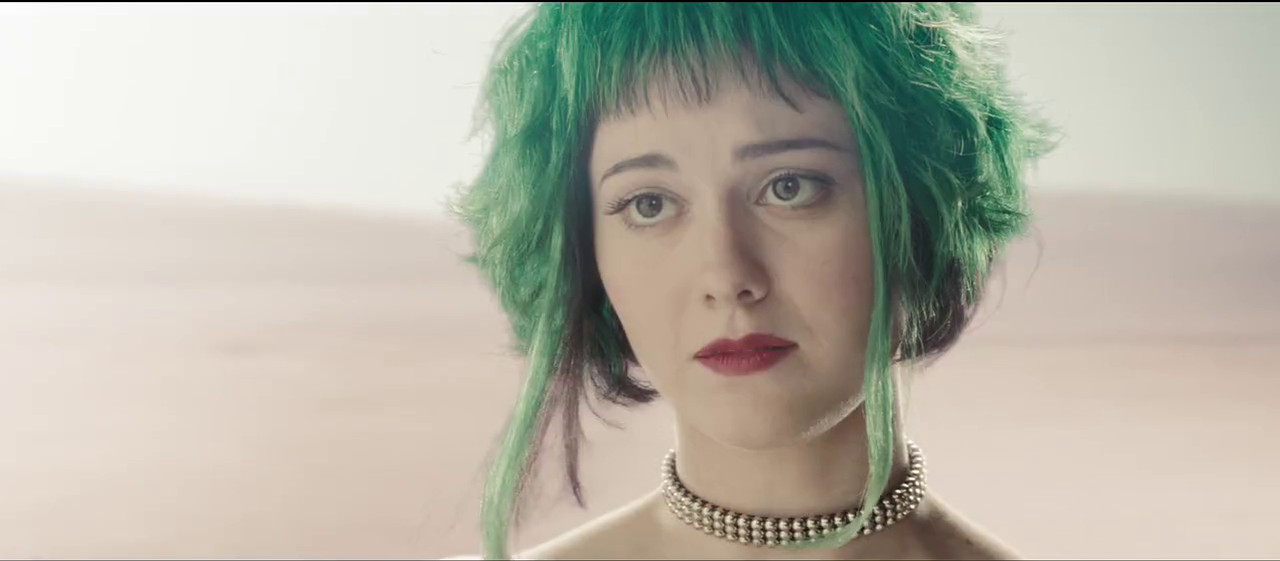
\includegraphics[width=\textwidth]{images/scott1}
        \caption{}
        \label{fig:images_scott1}
    \end{subfigure}
    \begin{subfigure}[b]{0.49\textwidth}
        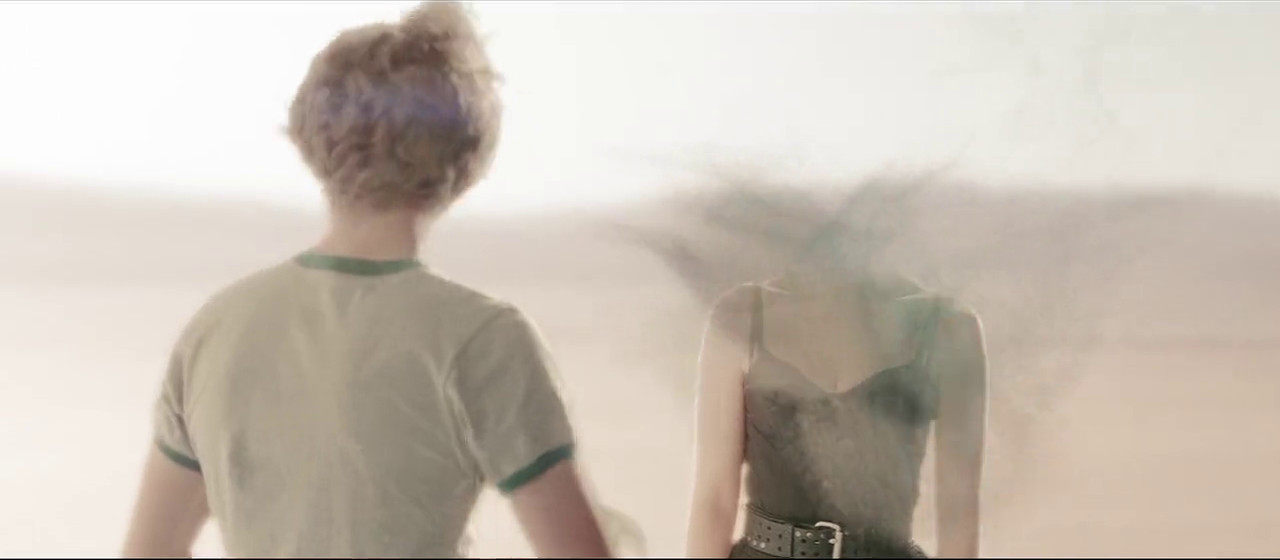
\includegraphics[width=\textwidth]{images/scott2}
        \caption{}
        \label{fig:images_scott2}
    \end{subfigure}
    \caption{Téléportation d'un personnage, \textit{Scott Pilgrim vs the world
             (2010)}, un film de \textit{Edgar Wright}}
\end{figure}

\end{document}
